% % % % % % % % % % % % % % % % % % % % % % % % % % % % % % % % % % % % % % % % 
% Formelsammlung von LaTeX4EI									
%
% @encode: 	UTF-8, tabwidth = 4, newline = LF
% @author:	Emanuel Regnath
% @date:		
%
% % % % % % % % % % % % % % % % % % % % % % % % % % % % % % % % % % % % % % % % 

%---------------------------------------%
%				Mathematik 4			%
%~~~~~~~~~~~~~~~~~~~~~~~~~~~~~~~~~~~~~~~%

% Document Class ===============================================================
\documentclass[fs, footer]{latex4ei}

% DOCUMENT_BEGIN ===============================================================
\begin{document}

\maketitle

% SECTION ======================================================================
\section{Nützliches Wissen $e^{\i x} = \cos (x) + \i \cdot \sin(x)$}
% ==============================================================================
\begin{sectionbox}
\subsection{Sinus, Cosinus \quad $\sin^2(x) \bs + \cos^2(x) = 1$}
\setlength{\tabcolsep}{4pt}
\begin{tablebox}{c|c|c|c|c||c|c|c|c} \ctrule
	$x$ & $0$ & $\pi / 6$ & $\pi / 4$ & $\pi / 3$ & $\frac{1}{2}\pi$ & $\pi$ & $1\frac{1}{2}\pi$ & $2 \pi$ \\
	$\scriptstyle{ \varphi }$ & $\scriptstyle{0^\circ}$ & $\scriptstyle{30^\circ}$ & $\scriptstyle{45^\circ}$ & $\scriptstyle{60^\circ}$ & $\scriptstyle{90^\circ}$ & $\scriptstyle{180^\circ}$ & $\scriptstyle{270^\circ}$ & $\scriptstyle{360^\circ}$ \\ \cmrule
	$\sin$ & $0$ & $\frac{1}{2}$ & $\frac{1}{\sqrt{2}}$ & $\frac{\sqrt 3}{2}$ & $1$ & $0$ & $-1$ & $0$ \\
	$\cos$ & $1$ & $\frac{\sqrt 3}{2}$ & $\frac{1}{\sqrt 2}$ & $\frac{1}{2}$ & $0$ & $-1$ & $0$ & $1$ \\     
	$\tan$ & $0$ & $\frac{\sqrt{3}}{3}$ &	$1$	&	$\sqrt{3}$ & $\pm \infty$ & $0$ & $\mp \infty$ & $0$\\ \cbrule
\end{tablebox}
\begin{tablebox}{\columnwidth}{@{\extracolsep\fill}ll@{}}
	Additionstheoreme &  Stammfunktionen\\
	$\cos (x - \frac{\pi}{2}) = \sin x$ & $\int x \cos(x) \diff x = \cos(x) + x \sin(x)$\\
	$\sin (x + \frac{\pi}{2}) = \cos x$ & $\int x \sin(x) \diff x = \sin(x) - x \cos(x)$\\
	$\sin 2x = 2 \sin x \cos x $  & $\int \sin^2(x) \diff x = \frac12 \bigl(x - \sin(x)\cos(x) \bigr)$\\ 
	$\cos 2x = 2\cos^2 x - 1$  & $\int \cos^2(x) \diff x = \frac12 \bigl(x + \sin(x)\cos(x) \bigr)$\\
	$\sin(x) = \tan(x)\cos(x)$ & $\int \cos(x)\sin(x) = -\frac12 \cos^2(x)$ \\
\end{tablebox}\\[1em]
\textbf{Sinus/Cosinus Hyperbolicus} $\sinh, \cosh$\\ 
% \quad \operatorname{arsinh}\ x:= \ln\left(x+\sqrt{x^2+1}\right) \\
\begin{tablebox}{\columnwidth}{@{\extracolsep\fill}ll@{}}
	$\sinh x = \frac{1}{2}(e^x -e^{-x})= - \i \, \sin(\i x)$ & $\cosh^2 x  \bs - \sinh^2 x = 1$\\
	$\cosh x  = \frac{1}{2}(e^x +e^{-x})= \cos(\i x)$ & $\cosh x + \sinh x = e^{x}$\\
\end{tablebox}\\
\textbf{Kardinalsinus} $\mathrm{si}(x) = \frac{\sin(x)}{x}$ \qquad genormt: $\sinc(x) = \frac{\sin(\pi x)}{\pi x}$
\end{sectionbox}

\begin{sectionbox}
\subsection{Integrale $\int e^x\;\mathrm{d} x = e^x = (e^x)'$}
Partielle Integration: $\int uw'=uw-\int u'w$\\
Substitution: $\int f(g(x)) g'(x)\,\mathrm dx=\int f(t)\, \mathrm dt$\\
\tablebox{
	\renewcommand{\arraystretch}{1.6} 
	\begin{tablebox}{\columnwidth}{@{\hspace{5mm}}c@{\extracolsep\fill}c@{\extracolsep\fill}c@{\hspace{5mm}}} \ctrule
		$F(x)$ & $f(x)$ & $f'(x)$ \\ \cmrule
		$\frac[0.1em]{1}{q+1}x^{q+1}$ & $x^q$ & $qx^{q-1}$ \\
		\raisebox{-0.2em}{$\frac[0.1em]{2\sqrt{ax^3}}{3}$} & $\sqrt{ax}$ & \raisebox{0.2em}{$\frac[0.1em]{a}{2\sqrt{ax}}$}\\
		$x\ln(ax) -x$ & $\ln(ax)$ & $\textstyle \frac{a}{x}$\\
		%e^x & e^x & e^x \\
		$\frac{1}{a^2} e^{ax}(ax- 1)$ & $x \cdot e^{ax}$ & $e^{ax}(ax+1)$ \\
		$\frac{a^x}{\ln(a)}$ & $a^x$ & $a^x \ln(a)$ \\
		$-\cos(x)$ & $\sin(x)$ & $\cos(x)$\\
		$\cosh(x)$ & $\sinh(x)$ & $\cosh(x)$\\
		$-\ln |\cos(x)|$ & $\tan(x)$ & $\frac[0.1em]{1}{\cos^2(x)}$ \\ \cbrule
	\end{tablebox} }\\
	
	$\int e^{at} \sin(bt) \diff t = e^{at} \frac{a \sin(bt) + b \cos(bt)}{a^2 + b^2}$\\
	\begin{tablebox}{\columnwidth}{@{\extracolsep\fill}ll@{}}
		$\int \frac{\diff t}{\sqrt{at+b}} = \frac{2 \sqrt{at+b}}{a}$ & $\int t^2 e^{at} \diff t = \frac{(ax-1)^2+1}{a^3} e^{at}$\\
		$\int t e^{at} \diff t = \frac{at-1}{a^2} e^{at}$ & $\int x e^{ax^2} \diff x = \frac{1}{2a} e^{ax^2}$\\
	\end{tablebox}
\end{sectionbox}

\begin{sectionbox}
	\subsection{Exponentialfunktion und Logarithmus}
	\begin{tablebox}{\columnwidth}{l@{\extracolsep\fill}ll}
		$a^x = e^{x \ln a}$ & $\log_a x = \frac{\ln x}{\ln a}$ & $\ln x \le x -1$\\
		$\ln(x^{a}) = a \ln(x)$ & $\ln(\frac{x}{a}) = \ln x - \ln a$ & $\log(1) = 0$\\
	\end{tablebox}
\end{sectionbox}

\begin{sectionbox}
	\subsection{Determinante von $A\in \mathbb K^{n\times n}$: $\det(A)=|A|$}
	$\det\begin{pmatrix}\ma A & \ma 0\\ \ma C&\ma D\end{pmatrix}=\det\begin{pmatrix}\ma A&\ma B\\\ma 0&\ma D\end{pmatrix}=\det(\ma A)\cdot\det(\ma D)$ \\
	Hat $\ma A$ 2 linear abhäng. Zeilen/Spalten $\Rightarrow |\ma A|=0$ \\
	Entwicklung. n. $i$ter Zeile: $|\ma A|=\sum\limits_{i=1}^n (-1)^{i+j} \cdot a_{ij} \cdot |\ma A_{ij}|$\\ 
	Inverse $2\times 2$: \quad $\mat{a & b\\ c & d}^{-1} = \frac{1}{ad-bc} \mat{d & -b\\ -c& a}$
}

\begin{sectionbox} $\i = \sqrt{-1}$ \qquad $|\cx z|^2 = \cx z \cxc z = x^2+y^2$ }

\begin{sectionbox}
	\subsection{Reihen}
	$\underset{\text{Harmonische Reihe}}{\sum\limits_{n=1}^\infty \frac{1}{n} \ra \infty} \qquad   \underset{\text{Geometrische Reihe}}{\sum\limits_{n=0}^\infty q^n \stackrel{|q|<1}= \frac{1}{1-q}}  \qquad \underset{\text{Exponentialreihe}}{\sum\limits_{n = 0}^{\infty} \frac{z^n}{n!} = e^z}$
\end{sectionbox}

\begin{sectionbox}
	\subsection{Wichtige Formeln}
	%noneed \setlength{\tabcolsep}{0pt}
	\tablebox{
		\begin{tablebox}{\columnwidth}{@{\extracolsep\fill}ll@{}} \ctrule
			Dreiecksungleichung: &$\big|\! \abs{x}- \abs{y}\!\big| \le \abs{x \pm y} \le \abs{x} + \abs{y}$\\
			Cauchy-Schwarz-Ungleichung: & $\left| \vec x^\top \bdot \vec y \right| \le \| \vec x\| \cdot \| \vec y\|$ \\
			Bernoulli-Ungleichung: & $(1+x)^n \ge 1+nx$\\ \cmrule
			Aritmetrische Summenformel &  $\sum \limits_{k=1}^{n} k = \frac{n (n+1)}{2} $ \\
			Geometrische Summenformel &  $ \sum \limits_{k=0}^{n} q^k = \frac{1 - q^{n+1}}{1-q}$ \\
			Binomialkoeffizient & $\binom nk = \binom n{n-k} = \frac{n!}{k! \cdot (n-k)!}$\\
			\ctrule
		\end{tablebox} }
	\end{sectionbox}

% =============================================================================================================
\section{Grundlagen der Numerik}
%$\delta f = f(x+\delta x) - f(x)$	
\begin{sectionbox}
	\subsection*{Begriffe:}
	\tablebox{
		\begin{tablebox}{\columnwidth}{@{\extracolsep\fill}lp{5cm}@{}}
			\ctrule
			Numerik & liefert eine zahlenmäßige Lösung eines Problems mit einem Algorithmus.\\
			Kondition & Ein Maß wie stark sich Eingabefehler auf die Ausgabe auswirken. $\kappa = \frac{\norm{\delta f}}{\norm{\delta x}} \ra |f'(x)|$\\
			$f(x)$ & Mathematisches Problem $f$ mit exakter Eingabe $x$\\
			$\tilde f(\tilde x)$ & Numerischer Algorithmus $\tilde f$ mit gerundeter Eingabe $\tilde x$\\
			\cbrule
		\end{tablebox}
	}
\end{sectionbox}

\begin{sectionbox}
	\subsection{Zahlen und Arithmetik im Rechner}
	Gleitkommazahlen nach IEEE 754: \quad $Wert = (-1)^s \cdot 2^{e-127} \cdot 1.f$\\
	$s \in \eset{-1;1}$: Vorzeichen, $e \in \mathbb Z$: Exponent, $f \in \N$: Mantisse\\ 
	\\
	Gleitpunktzahlen: \\
	$\mathbb G_{b,t} = \iset{ x \in \mathbb G_{b,t}}{e_{\ir min} \le e_{\ir max}} \cup \eset{\pm \infty, \text{NaN}}$ \\
	
	Maschinenzahlen:\\
	$\mathbb M_{b, t, e_{\ir min}, e_{\ir max}} = \iset{x \in \mathbb G_{b,t}}{e_{\ir min} \le e \le e_{\ir max}} \cup \eset{\pm \infty, \text{NaN}}$ \\
	Anzahl der Maschinenzahlen $| \mathbb M | = 2a(b-1)b^{t-1} + 1$\\
	
	Maschinengenauigkeit $\epsilon_{b,t} = b^{-(t-1)}$\\
	In MATLAB: $\epsilon_{2,53} \approx \SI{2e-16}{}$ \qquad Runden: $fl_{b,t}(x)$\\
\end{sectionbox}

\begin{sectionbox}
	\subsection{Kondition:}
	$\kappa_{\ir abs}(x) = \abs{f'(x)}$ \qquad\qquad $\kappa_{\ir rel}(x) = \frac{\abs{f'(x)} \cdot \abs{x}}{\abs{f(x)}}$\\
	Falls $\kappa_{\ir rel} \ll 100$: gute Konditionierung\\
	\\
	Verkettung $h = g(f(x))$ \quad $\kappa^h_{\ir abs}(x) = \kappa^g_{\ir abs}(f(x))\kappa^f_{\ir abs}(x)$\\
\end{sectionbox}

\begin{sectionbox}
	\subsection{Fehler}
	Absolut: $\norm{\tilde f(x) - f(x)}$ \qquad\qquad Relativ: $\frac{\norm{\tilde f(x) - f(x)}}{\norm{f(x)}}$
\end{sectionbox}

\begin{sectionbox}
	\subsection{Stabilität}
	$\forall x \in X \quad \land \quad \tilde x:\frac{\norm{x-\tilde x}}{\norm{x}} = \mathcal O(\epsilon_{b,t})$\\
	Vorwärtsstabil:  $\frac{\norm{\tilde f(x) - f(\tilde x)}}{\norm{f(x)}} = \mathcal{O}(\epsilon_{b,t})$\\
	Rückwärtsstabil: $\forall x \in X:\tilde f(x) = f(\tilde x)$\\
	\\
	Horna-Schema für Polynome: $(...((a_n) x + a_{n-1})x + ... +a_{1})x + a_0$\\
\end{sectionbox}	

% =============================================================================================================
\section{Matrix Zerlegung}
\begin{sectionbox}
	\subsection{LR-Zerlegung von Matrizen (\textbf{L}ower and \textbf{U}pper)}
	Geeignetes Lösungsverfahren für $\ma A \vec x = \vec b$, falls $n < 500$\\ 
	$\ma A = \ma L \cdot \ma R$ \quad mit $\ma R$ ist obere Dreiecksmatrix\\
	\cookbox{Gaußverfahren durch Matrixmultiplikaiton}{
		\item Zerlegen des Problems $\ma A \vec x = \vec b$ in das Problem $\ma L (\ma R \vec x) = \vec b$  mit $\ma A = \ma L \ma R$ bzw. $\ma L \vec y = \ma P \vec b$ (mit Pivotisierung)
		\item Zerlegungsmatrix (für $2 \times 2$): \\ $\ma A = \mat{a & b \\ c & d} \ra \mat{a & b \\ \frac{c}{a} & d - \frac{c}{a} b} = \ma A^*$ mit den Eliminationsfaktoren $l_{ik} = \frac{a_{ik}}{a_{kk}} \overset{z.B.}{=} \frac{c}{a}$
		\item Für jede Spalte der unteren Dreiecksmatrix wiederholen.\\
		Für eine $3 \times 3$ Matrix bräuchte man 2 Durchläufe, da 3 Spalten Elimationsfaktoren bestimmt werden müssen.
		\item $\ma R = \text{triu}(\ma A^*)$\\
		(obere Dreiecksmatrix von $\ma A^*$, inkl. Diagonalelemente)
		\item $\ma L = \text{tril}(\ma A^*,-1)+\ma 1$\\
		(untere Dreiecksmatrix mit $1$en auf der Diagonale.
		
		%$\ma A = \mat{ \alpha & \vec u^\top \\ \vec v & \ma A'} = \mat{1 & 0 \\ \vec w & \ma L} \cdot \mat{ \alpha & \vec u^\top \\ w & \ma R}$\\
		%$\mat{a & b & c\\ d & e & f\\ g & h i} \ra \mat{a & b & c\\ \frac{d}{a} & e - \frac{d}{a} b & f - \frac{d}{a} c \\ }$
		\item Vorwärtseinsetzen: $\ma L \vec y = \vec b$ bzw. $\ma L \vec y = \ma P \vec b$ (mit Pivotisierung)\quad (Löse nach $\vec y$)
		\item Rückwärtseinsetzen: $\ma R \vec x = \vec y$ \quad (Löse nach $\vec x$)
		
	} \\
	
	
	\subsubsection{Pivotisierung (Spaltenpivotsuche)}
	Permutationsmatrix $\ma P^\top = \ma P^{-1}$ vertauscht Zeilen, damit LR Zerlegung bei 0 Einträgen möglich ist.
	Tausche so, dass man durch die betragsmäßig größte Zahl dividiert (Pivoelement) %Verhindert Auslöschung
\end{sectionbox}

\begin{sectionbox}
	\subsection{QR-Zerlegung}
	$\ma A = \ma Q \ma R$ mit $\ma Q^{-1} = \ma Q^\top$\\	
	Verfahren: Housholder (numerisch stabil) , Gram-Schmidt, Givens Rotation.\\
	$\ma A \xrightarrow{EZF} \ma H\ma A \xrightarrow{EZF} \tilde{\ma H} \ma H \ma A = \ma R \Ra \ma A = \ma H^\top \tilde{\ma H}^\top \ma R$\\
	Aufgabe: Finde Vektor $\vec v$ der Senkrecht auf $\ma H$ steht.\\
	\\
	\cookbox{Q/R Zerlegung für $\ma A \in \mathbb R^{m\times n }$}{
		\item Setze $\vec a = \vec s_1$ (erste Spalte) und $\vec v = \vec a + \sgn ( a_1) \norm{\vec a} \vec e_1$
		\item Konstruiere die \emph{Householder} Transformationsmatrix mit \\
		$\ma H_v = \ma E_m - \frac{2}{\vec v^\top \vec v} \vec v \vec v^\top$
		\item Erhalte die Matrix $\ma H_v \ma A$ die in der ersten Spalte bis auf das Element $a_{11}$ nur Nullen enthält
		\item Setze $\ma Q_1 = \ma H_v$ 
		\item Wende den gleichen Algorithmus auf die Untermatrix $\ma A^*$ ($\ma H_v \ma A$ ohne erste Zeile und Spalte) an.
		\item Setze anschließend $\ma Q_2 = \ma H_v$ und fülle mit erweitere mit $E_m$ (d.h. erste Zeile und Spalte die von $E_m$)
		\item Nach $p = \min \eset{m - 1, n}$ Schritten: $\ma H_v \ma A^*$ ist obere Dreiecksmatrix $\ra $ Disco, disco, party, party $;)$
		\item Somit ist mit $\ma Q^\top = \ma Q_p \cdots \ma Q_1$ ist $\ma Q^\top \ma A = \ma R$ und $\ma A = \ma Q \ma R$
	}
	
	\subsubsection*{Anwendungen}
	\paragraph{Lösen von LGSen mit der $Q R$ Zerlegung}
	Bestimme $\vec x$ durch Rückwärtssubsitution aus $\ma R \vec x = \ma Q^\top \vec b$
	\paragraph{Anwendung in der linearen Ausgleichsrechnung}
	(Minimierung d. Restes)\\
	Problem: $\ma A^\top \ma A \vec x = \ma A^\top \vec b$ mit $\ma A \in \mathbb R^{m \times n }$ und $\vec b \in \mathbb R^{m}$ \\ 
	\cookbox{Lösen der Normalengleichung}{
		\item Bestimme eine reduzierte QR-Zerlegung \\ $\ma A = \tilde{\ma Q}  \tilde{\ma R}$ mit $\tilde{\ma Q} \in \mathbb R^{m \times n}, \tilde{\ma R} \in \mathbb R^{n \times n}$
		\item Löse $\tilde{\ma R } \vec x =\tilde{\ma Q}^\top \vec b$
	}
	$\norm{\vec b - \ma A \vec x}^2 = \norm{\ma Q^\top (\vec b - \ma A \vec x)}^2 = \norm{\tilde{\vec b} - \tilde{\ma R} \vec x}^2 + \norm{\vec c}^2 \ge \norm{\vec c^2}$
	%ML: a=A(1:end,1); alpha = -sign(a(1)).*norm(a); H = eye(size(A)) - 
\end{sectionbox}
% =============================================================================================================
\section{Fixpunktiteration}

\begin{sectionbox}
	Nullstellenproblem $f(x) = 0$\\
	Fixpunktproblem $\phi(x) = x$ \qquad mit $\phi(x) = g(x)f(x) + x$\\  %\phi' muss kleiner 1 sein
	Rekursive Lösung: \boxed{ x_{i+1} = \phi(x) }\\
	\\
	Bsp: $x^7 - x -2$ \quad $x = \sqrt[7]{x+2}, x= x^7 -2$\\ 
	MATLAB: \texttt{x=s; for k=1:n; x=phi(x); end}
	
	\subsection{Konvergenz von Iterationsverfahren}
	Falls $(x_k)_k$ mit $x_0 = s$ und $x_{k+1} = \phi(x_k)$ dann ist der Grenzwert von $(x_k)_k$ ein Fixpunkt von $\phi$,
	denn $x = \lim\limits_{k \ra \infty} \phi(x_k) = \phi(\lim\limits_{k \ra \infty} x_k) = \phi(x)$\\
	Fehler $e_k = |x_k - x_*|$\\
	Libschitzstetig: $\exists L < \infty:\norm{f(a)-f(b)} \le L \norm{a-b}$\\
	\textbf{Globaler Konvergenzsatz von Banach für $\phi:D\ra\R^n$} \\
	Falls \begin{itemize}\itemsep0pt
		\item $D \subseteq \mathbb R^n$ ist abgeschlossen
		\item $f(D) \subseteq D$ (Selbstabbildung)
		\item $\exists L = \sup\limits_{x\in D} \norm{\phi'(x)} < 1$ \quad (Kontraktion)\\
	\end{itemize}
	Dann konvergiert $\phi$ $\forall x_0 \in D$ eindeutig gegen $x_*$ und es gilt folgende Fehlerabschätzung:
	\begin{itemize}\itemsep1pt
		\item A-Priori: $\norm{x_k - x_*} \le \frac{L^k}{1 - L} \norm{x_1 -x_0} \le \varepsilon$
		\item A-posteriori: $\norm{x_k - x_*} \le \frac{L}{1 - L} \norm{x_k -x_{k-1}}$
		\item Für Genauigkeit $\varepsilon$: $k \ge \ln\left( \frac{\varepsilon(1-L)}{\norm{x_1 -x_0}}\right) / \ln(L)$
	\end{itemize}
	\textbf{Lokale Konvergenz:} $\phi([a,b]) \subseteq [a,b] \quad \land \quad \abs{\phi'([a,b])} < 1$\\
	\textbf{Lokale Konvergenz ohne Norm:} Falls $\max{\lambda_i} < 1$ mit $\lambda_i$ is EW von $\ma J_\phi$\\
\end{sectionbox}

% SECTION =============================================================================================================	
\section{Iterative Näherungsverfahren}
\begin{sectionbox}
	\subsection*{Problemstellung}
	Schreibe $\ma A \vec x = \vec b$ in ein Fixpunktproblem um:\\
	Finde $\ma A = \ma M - \ma N$ mit $\ma M$ ist invertierbar. \quad $\Ra (\ma M - \ma N)\vec x = \vec b$\\
	\boxed{ \phi(\vec x) = \ma M^{-1} \ma N \vec x + \ma M^{-1} \vec b = \ma T \vec x + \ma C }\\
	\\
	Für jedes $x_0 \in \R^n$ konvergent, falls Spektralradius $\rho(\ma M^{-1}\ma N) < 1$\\
	Je kleiner der Spektralradius von $\ma M^{-1}\ma N$ desto bessere Konvergenz.\\
	\\
	\tablebox{
		\begin{tablebox}{\columnwidth}{@{\extracolsep\fill}ll@{}}
			\ctrule
			$\ma A = \ma M - \ma N$ & Systemmatrix\\
			$\ma D$ & Diagonalmatrix \texttt{diag(diag($\ma A$))}  \\
			%$\ma N = \ma L + \ma R = \ma D - \ma A$\\
			$\ma L$ & negative linke untere Dreiecksmatrix \\
			$\ma R$ & negative rechte obere Dreiecksmatrix \\
			\ctrule
		\end{tablebox}
	}
\end{sectionbox}

\begin{sectionbox}
	\subsection*{Wichtige Begriffe}
	\textbf{Diagonaldominante Matrix:} Diagonalelemente sind größer als die restlichen Elemente der selben Zeile: $|a_{ii}| > \sum_{j} |a_{ij}|$ mit $j \ne i$\\
	\textbf{Spektralradius $\rho(\ma A)$ einer Matrix $\ma A$:} Betragsmäßig größter Eigenwert. \\
	Konvergenzbeweis aller Verfahren: Gershgorinkreise um die Null mit $r \le 1$
\end{sectionbox}

\begin{sectionbox}
	\subsection{Jacobiverfahren}
	Konvergiert $\forall x_0 \in \R^n$, falls $\ma A$ strikt diagonaldominant.\\
	$\vec x_0 = s \in \R^n$ \qquad $\ma M = \ma D$ \qquad $\ma N = \ma L + \ma R = \ma D - \ma A$\\
	\boxed{ \vec x_{k+1} = \phi(\vec x_k) = \ma D^{-1} \bdot (\ma D - \ma A) \bdot \vec x_k + \ma D^{-1} \vec b }\\
	Komponentenweise: $\vec x_{k+1} = (a^{-1}_{ii}(b_i - \sum\limits_{j = 1, j \ne i} a_{ij} x_{k,j} )_i$
\end{sectionbox}

\begin{sectionbox}
	\subsection{Gauß-Seidel Verfahren}
	Unterschied zu Jacobi: Komponentenweise Berechnung von $\vec x$ mit bereits iterierten Werten. (Kürzere Iterationszyklen)\\[0.5em]
	\emph{Konvergenz:} $\ma A$ ist strikt diagonaldominant \textbf{oder} $\ma A$ ist positiv definint.\\
	\emph{Komponentenweise Darstellung:} \\ \boxed{ \vec x_i^{(k+1)} = a^{-1}_{ii} \left( b_i - \sum\limits_{j = 1}^{i-1} a_{ij} x^{(k+1)}_j - \sum\limits_{j=i+1}^n a_{ij} x^{(k)}_j \right) }\\
	\\
	\emph{Matrixdarstellung:}\\
	\boxed{ \vec x^{(k+1)} = (\ma D - \ma L)^{-1} \bdot \big( \ma R \vec x^{(k)} + \vec b\big) }\\[0.5em]
	Mit $\ma M = (\ma D - \ma L)$ \qquad $\ma N = \ma R$
\end{sectionbox}

\begin{sectionbox}
	\subsection{SOR Verfahren}
	\emph{Konvergenz:} für $0  < \omega < 2$ und positiv definites $\ma A$\\
	\boxed{ \vec x^{(neu)}_{k+1} = \omega \vec x^{(alt)}_{k+1} + (1-\omega) \vec x_k }\\ %\quad \boxed{ \phi_\omega(\vec x) = \omega \phi(\vec x) + (1-\omega)\vec x}\\
	Bestimme $\omega$ so, dass die Konvergenz besser wird: $\omega_{opt} = \frac{2}{2 - \lambda_1 - \lambda_2}$\\
	
	
	\emph{Matrixdarstellung:}\\
	$\vec x_{k+1} = (\ma 1_n - \omega \ma D^{-1} \ma L)^{-1} (( 1 - \omega) \ma 1_n + \omega \ma D^{-1} \ma R) x_k + \omega (1_n - \omega \ma D^{-1} \ma L)^{-1} \ma D^{-1} \vec b$ \\
	$\ma A = (\frac{1}{\omega} \ma D - \ma L) - \left((\frac{1}{\omega} - 1) \ma D + \ma R \right)$\\
	
	\emph{Komponentendarstellung:}\\
	$x_i^{k+1} = \omega a_{ii}^{-1} \left( \vec b_i - \sum\limits_{j=1}^{i-1} a_{ij} x_j^{(k+1)} - \sum\limits_{j = i +1}^{n} a_{ij} x_j^{(k)} \right) + (1 - \omega) x_i^{(k)}$
\end{sectionbox}


% Heute: Krylow Unterraumverfahren
% Googlematrix: So viele Zeilen wie es Webseiten gibt
%Satz von Gershgorin: Alle Eigenwerte 


% MATLAB:
%relerr = inf; niter =1;
% while relerr >= tol & iter < maxiter; x=M




%ML: x = M\(Nx+b), D = diag(diag(A))
% Faustregel: 50 Iterationen für 15 genaue Stellen bei lin. konvergenz

% SECTION =============================================================================================================	
\section{Nichtlineare Gleichungen}
\begin{sectionbox}
	\subsection*{Problemstellung}
	Gegeben nichtlineare, stetige Funktion \\ 
	$f: [a_0, b_0] \ra \R, f(a_0)\cdot f(b_0) < 0$
\end{sectionbox} \\ \\

\begin{sectionbox}
	\subsection{Bisektionsverfahren}
	Globale, lineare Konvergenz mit $|x^* - x_k| \le \frac{1}{2^k} (b_0 -a_0)$\\
	\cookbox{Bisektionsverfahren}{\item $x_k = \frac{1}{2}(a_k + b_k)$
		\item $\begin{array}{rl} a_{k+1} = a_k,\ b_{k+1} = x_k & \text{, falls } f(a_k)f(x_k) < 0 \\ a_{k+1} = x_k,\ b_{k+1} = b_k & \text{, sonst} \end{array}$
		\item Abbruch falls $|b_k - a_k| < \varepsilon$ oder maxiter erreicht}
\end{sectionbox}

\begin{sectionbox}
	\subsection{Newton-Raphson-Verfahren}
	Funktion durch Gerade annähern und Nullstelle bestimmen. An dieser Stelle den Vorgang wiederholen.
	Nur geeignet für einfache Nullstellen.\\
	$\exists$ Umgebung $U$ mit $f'(x) \ne 0 \forall x \in U$\\
	\boxed{ x_{k+1} = x_k - \frac{f(x_k)}{f'(x_k)} } \\
	\boxed{ \vec x_{k+1} = \vec x_k - \ma J_{\vec f}^{-1}(\vec x_k) \vec f(\vec x_k) } \qquad
	\parbox{4cm}{MATLAB: \\ $x = x - \ma J_{\vec f}$\textbackslash $f$}\\
	Abbruchkriterium: $\norm{\vec x_k - \vec x^*} \le \norm{\Delta \vec x} + c \norm{\vec x_k - \vec x^*}$
	\subsubsection{Vereinfachtes Newtonverfahren}
	Man benutzt die Jacobimatrix über mehrer Iterationen. \\
	\textbf{Bemerkungen:} Es gibt keine Existenz und Eindeutigkeitsaussage zur Lösbarkeit des Nullstellenproblems \\ 
	\emphbox{$\ma J_f (x) = \begin{bmatrix} \frac{\partial f_1}{\partial x_1} & \frac{\partial f_1}{\partial x_2} \\ \frac{\partial f_2}{\partial x_1} & \frac{\partial f_2}{\partial x_2} \end{bmatrix}$
	}
\end{sectionbox}

% SECTION =============================================================================================================	
\section{Numerik gewöhnlicher DGL}
$\dot x(t) = f\big(t,x(t)\big),\quad x(t_0) = x_0$ \qquad Samples $h = \frac{t-t_0}{n}$\\
Vorgehen: Finde diskrete Werte $x[t_i]$ anstatt Näherungsfunktion $x = x(t)$\\

\begin{sectionbox}
	\subsection{Einzelschrittverfahren}
	Def: Man erhält $x_{k+1}$ aus $x_k$\\
	\textbf{Eulersches Polygonzugverfahren:} $x_{k+1} = x_k + h \cdot f(t_k,x_k)$\\
	\textbf{Mittelpunktregel} (implizit): \\ $x_{k+1} = x_k + h \cdot f(\frac{t_{k+1}+t_k}{2},\frac{x_{k+1}+x_k}{2})$\\
	\textbf{Implizites Eulerverfahren} (rekursiv): $x_{k+1} = x_k + h \cdot f(t_{k+1},x_{k+1})$\\
	\\
	Mit verkleinern der Schrittweite wird die Genauigkeit der Lösung nicht unbedingt besser (Schrittweitensteuerung)
	
	Mehrschrittverfahren: Man erhält $x_{k+1}$ aus $x_k, x_{k-1}, ... x_1$
\end{sectionbox}

\section{Verfahren zum numerischen Lösen von DGLs}

\begin{sectionbox}
	\subsection{4 Stufiges Runge-Kutta Verfahren}
	Einschrittverfahren für AWPs mit variabler Schrittweite.\\
	Butcher Schema: $\begin{array}{c|c} \vec c & \ma A \\ \mrule & \vec b^\top \end{array} =$
	$\left. \begin{matrix}0 \\ \frac 1 2 \\ \frac 1 2 \\ 1 \\ \text{}\end{matrix} \right| \begin{matrix}0 & 0 & 0 & 0 \\ \frac 1 2 & 0 & 0 & 0 \\ 0 & \frac 1 2 & 0 & 0 \\ 0 & 0 & 1 & 0 \\ \frac 1 6 & \frac 1 3 & \frac 1 3 & \frac 1 6\end{matrix}$ \\ \\ \\
	\begin{tablebox}{@{}ll}
		$k_1 =f( t_n, x_n)$ & $k_3 = f(t_n + \frac h 2, x_n + \frac h 2 k_2)$\\
		$k_2 = f(t_n + \frac h 2 , x_n + \frac h 2 k_1) $ & $k_4 = f(t_n + h , x_n + h k_3)$\\
	\end{tablebox}\\[0.5em]
	$x_{k+1} = x_k + h \sum b_i k_i = x_k + \frac{h}{6}\big(k_1 + 2(k_2 + k_3) + k_4\big)$ \\
	
	Für andere Stufenzahl($s$): $k_i = f(t_n + c_i h, x_n + h \sum \limits_{j=1}^s a_{ij} k_j)$
\end{sectionbox}

% SECTION =============================================================================================================	
\section{Optimierung}
\begin{sectionbox}
	\subsection*{Problemstellung}
	$\underset{\text{Zielfunktion}}{f:} \underset{\text{Zulässigkeitsbereich}}{X} \subseteq \R^d \ra \R$\\
	gesucht: $\min f = \max -f$\\
	$\nabla f(\vec x^*) = 0$ und $\ma H_f(\vec x^*)$ pos. definit. (Numerische Katastrophe)
\end{sectionbox} \\ \\

\begin{sectionbox}
	\subsection{Abstiegsverfahren / Gradientenverfahren}
	Konvergenz: linear \\ 
	\cookbox{Abstiegsverfahren}{
		\item Bestimme Abstiegsrichtung $\vec v_k: \nabla f(\vec x_k)\vec v_k < 0$\\
		Gradientenverfahren: $\vec v_k = - \nabla f(\vec x_k)$
		\item Bestimme Schrittweite $\vec h_k: f(\vec x_k +  h_k \vec v_k) < f(\vec x_k)$\\
		Armijo: $\max h_k \in \eset{1,\frac12,\frac14,\frac18,...}$\\
		$f(\vec x_k + h_k \vec v_k) < f(x_k) + h_k \gamma \nabla f(\vec x_k)^\top \vec v_k$ \quad $\gamma \in ]0,1[$
		\item Setze $\vec x_{k+1} = \vec x_k +  h_k \vec v_k$
		\item Abbruch, falls $\vec x_k$ approximativ stationär ist.
	} \\ 
\end{sectionbox}

\begin{sectionbox}
	\subsection{Das lokale Newton-Optimierungsverfahren}
	Geg: $f \in \mathcal C^2$, Ges: $\vec x^*:\nabla f(\vec x^*) = 0$ \\ \\ 
	\cookbox{lokales Newton-Optimierungsverfahren}{
		\item Wähle Startpunkt $x_0 \in \mathbb R^d$
		\item Falls $\nabla f(x_k) = 0$ $\ra$ Stop: Ergebnis $x_k$
		\item Bestimme $\vec v_k$ durch lösen von $\ma H_f(\vec x_k) \vec v_k = -\nabla f(\vec x_k)$
		\item Setze $\vec x_{k+1} = \vec x_k + \vec v_k$
	}
\end{sectionbox}

\begin{sectionbox}
	\subsection{Das globale Newton-Optimierungsverfahren}
	Geg: $f \in \mathcal C^2$, Ges: $\vec x^*:\nabla f(\vec x^*) = 0$\\ \\ 
	\cookbox{globales Newton-Optimierungsverfahren}{
		\item Bestimme $\vec v_k$ durch lösen von $\ma H_f(\vec x_k) \vec v_k = -\nabla f(\vec x_k)$\\
		Falls $\nabla f(\vec x_k)^\top \vec v_k \ll 0 \ra$ Newtonschritt\\
		Falls $\nabla f(\vec x_k)^\top \vec v_k \not \ll 0 \ra$ Gradientenverfahren mit Armijo
		\item Setze $\vec x_{k+1} = \vec x_k + \vec v_k$
		\item Abbruch, falls $\vec x_k$ approximativ stationär ist.
	}
\end{sectionbox}

% SECTION =============================================================================================================	
\section{Funktionentheorie (Komplexe Funktionen)}
\begin{sectionbox}
	\subsection{Reelifizierung}
	\pbox{6cm}{
		$\cx f(\cx z) = \cx f(x+y \i) = u(x,y) + \i v(x,y)$\\
		\\
		$\sin(\cx z) = \sin(x)\cosh(y) + \i \cos(x)\sinh(y)$\\
		$\cos(\cx z) = \cos(x)\cosh(y) - \i \sin(x)\sinh(y)$\\
		\\
		$\sinh(\cx z) = \cos(y) \sinh(x) + \i \sin(y) \cosh(x)$\\
		$\cosh(\cx z) = \cos(y) \cosh(x) + \i \sin(y) \sinh(x)$ }\ 
	\pbox{4cm}{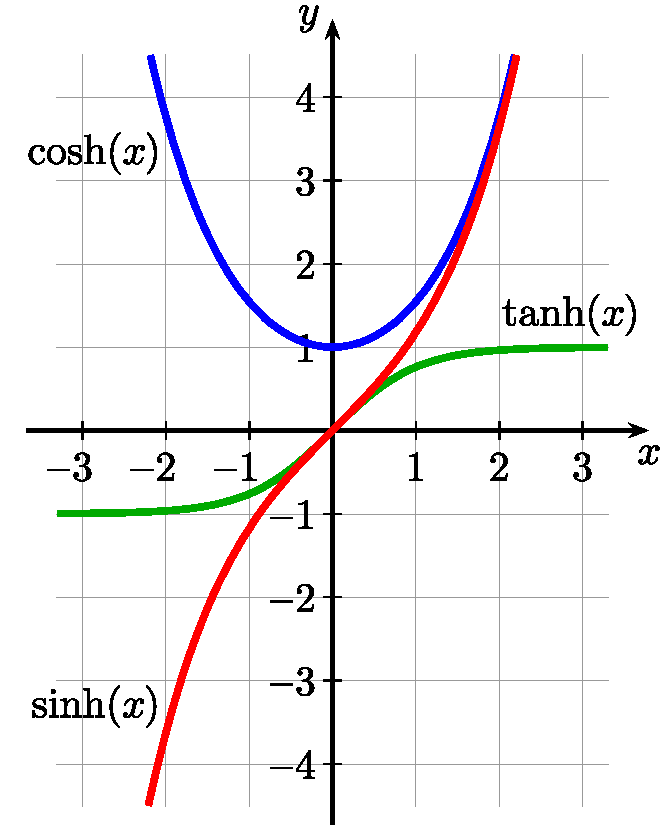
\includegraphics[width = 2cm]{./hyperbolis.pdf} }
\end{sectionbox}

\begin{sectionbox}
	\subsection{holomorphe(analytische, reguläre) Funktionen $\cx f$}
	Eine Funktion $\cx f$ ist \\ 
	\tablebox{
		\begin{tablebox}{\columnwidth}{@{\extracolsep\fill}ll@{}}
			\ctrule
			holomorph & falls $\cx f$ in $G$ komplex differenzierbar ist.\\
			ganz & falls $\cx f$ in ganz $\C$ komplex differenzierbar ist.\\
			konform & falls Kurven Winkel- und Orientierungstreu bleiben.\\
			\ctrule
		\end{tablebox}
	}
	$\cx f$ ist genau dann holomorph, falls $f(x+y\i) = u(x,y) + \i v(x,y)$ und
	\begin{itemize}\itemsep0pt
		\item $u,v$ sind stetig partiell diffbar
		\item Cauchy-Riemann DGLs sind erfüllt:\\
		$\partial_x u(x,y) = \partial_y v(x,y)$ \qquad $\partial_y u(x,y) = - \partial_x v(x,y)$\\
	\end{itemize}
	Holomorph: $\exp, \sin, \cosh$, Polynome, $\cx f\pm \cx g, \cx f \cx g, \frac{\cx f}{\cx g}, \cx f(\cx g)$
\end{sectionbox}

\begin{sectionbox}
	\subsection{harmonische Funktionen $u,v$}
	$u$ bzw. $v$ sind harmonisch, falls gilt:\\
	$\lpo u = \partial_{xx} u + \partial_{yy} u = 0$ \qquad\quad $\lpo v = \partial_{xx} v + \partial_{yy} v = 0$\\[0.5em]
	oder falls $f(\cx z) = u + \i v$ holomorph ist; denn mit Satz von Schwarz:\\
	$\lpo u = \partial_{yx} v - \partial_{xy} v = 0$ \qquad\quad $\lpo v = - \partial_{yx} u + \partial_{xy} u = 0$\\
	\\
	\cookbox{Bestimmung der harmonischen Konjugierten}{
		\begin{itemize}
			\item geg: harm. Fkt. $u: G \ra \mathbb R, (x,y) \ra u(x,y)$
			\item ges: harm. Fkt. $v: G \ra \mathbb R, (x,y) \ra v(x,y)$
			so, dass $f: G \ra \mathbb V, f(z) = u(x,y) + \i v (x,y)$
			\item $v(x,y) = \int u_x \diff y$ mit Integrationskonstante $g(x)$
			\item $v_x = -u_y \Ra g'(x)$
			\item $g(x) = \int g'(x) \diff x \Ra v$ bis auf Konstante $C$ bestimmt
			\item zugehörige holomorphe Fkt.
			$f (z) = u (x,y) + \i v(x,y)$
		\end{itemize}
	}
\end{sectionbox}

\begin{sectionbox}
	\subsection{Möbiustransformation $\hat \C = \C \cup \eset{\infty}$}
	Einzige bijektive, holomorphe, konforme Abbildung von $\hat \C$ auf sich selbst.\\
	$\cx f:\C \setminus \eset{-\frac{d}{c}} \ra \C \setminus \eset{-\frac{d}{c}}, \cx f(\cx z) = \frac{a\cx z + b}{c\cx z + d}$ \qquad $ad - bc \ne 0$\\ 
	$\cx f^{-1}(\cx w) = \frac{d\cx w - b}{-c \cx w + a}$
\end{sectionbox}

\begin{sectionbox}
	\subsection{Komplexes Kurvenintegral}
	für $D \subset \mathbb C$ Gebiet, $f: D \ra \mathbb C$ stetig, $\cx \gamma: [t_1, t_2] \ra $ stetig diffbar orientierte Kurve. \\ 
	\cookbox{So brechnet man ein komplexes Kurvenintegral}{
		\item Bestimme Parametrisierung von $\cx \gamma$ \\
		$\cx \gamma = \cx \gamma_1 + \ldots + \cx \gamma_2$, $\cx \gamma_i : [a_i, b_i] \ra \C$
		\item Stelle Inegrale auf \\
		$\int_{\cx \gamma_i} \cx f(\cx z) \diff \cx z = \int \limits_{a_i}^{b_i} \cx f\big(\cx \gamma_i(t)\big) \cdot \dot{\cx \gamma}_i (t) \diff t$\\
		Falls $\cx f$ holomorph: $\int_{\cx \gamma} \cx f(\cx z) \diff \cx z = \cx F\big(\cx \gamma(b)\big) - \cx F\big(\cx \gamma(a)\big)$
		\item Berechne die Integrale und addiere: \\
		$\int \limits_{\cx \gamma} \cx f(z\cx ) \diff \cx z = \sum \limits_{i = 1}^{h} \int_{\cx \gamma_i} \cx f(\cx z) \diff \cx z$
	}
\end{sectionbox}

\begin{sectionbox}
	\subsection{Cauchy-Integralformel}
	(falls Unstetigkeitsstelle auf Gebiet $G$)
	Falls $\cx \gamma$ geschl. doppelpunktfreie Kurve in einfach zsh. Gebiet $G$ mit holomorphen Fkt. $\cx f$, gilt für jedes $\cx z_0 \in G$\\
	\boxed{\cx f(\cx z_0) = \frac{1}{2\pi \i} \ointctrclockwise_{\cx \gamma} \frac{\cx f(\cx z)}{\cx z - \cx z_0} \diff \cx z }\\
	$\cx f^{(k)}(\cx z_0) = \frac{k!}{2\pi \i} \oint_{\cx \gamma} \frac{\cx f(\cx z)}{(\cx z - \cx z_0)^{k+1}} \diff \cx z$ 
	
	\subsection{Integralsatz von Cauchy}
	Falls keine Unstetigkeitsstelle innerhalb der Kurve $\cx \gamma$\\ 
	$\cx f: G \ra \C$ komplex diffbar auf offenem, einfach zusammenhängendem Gebiet $G \subset \C$. $\cx \gamma$ sei einfach geschlossene Kurve in $G$ (keine Doppelpunkte). \\
	$\oint \limits_{\cx \gamma} \cx f(\cx z) \diff \cx z = 0$
\end{sectionbox}

\begin{sectionbox}
	\subsection{Singularitäten}
	Isolierte Singularität $\cx z_0$: \quad $\cx f :G \setminus \eset{\cx z_0} \ra \C$ \ (einzelne Punkte)\\
	Hebbare Sing., falls $f$ auf punktierter Umgebung beschränkt ist.\\
	Pol $m$ter Ordnung: $(\cx z - \cx z_o)^m \cx f(\cx z)$ ist hebbar in $\cx z_0$\\
	Wesentliche Singularität: Sonst.
\end{sectionbox}

\begin{sectionbox}
	\subsection{Taylorreihe und Laurentreihe}
	\emph{Taylorreihe:} falls $\cx f$ holomorph:\\
	\boxed{ \cx f(\cx z) = \sum\limits_{k = 0}^{\infty} \frac{\cx f^{(k)} \cx z_0}{k!} (\cx z - \cx z_0)^k }\\
	\\
	\emph{Laurentreihe:} Falls $\cx f$ nicht holomorph ist.\\
	\boxed{\sum\limits_{k = -\infty}^\infty \cx c_k (\cx z - \cx z_0)^k} \\
	zerfällt in $\sum \limits_{k=1}^{\infty} d_k w^k$ mit $d_k = c_{-k}$ und $w = \frac{1}{z - z_0}$ (Hauptteil) und $\sum \limits_{k = 0}^{\infty} c_k (z-z_0)^k$ (Nebenteil) \\
	Konvergenz falls Hauptteil und Nebenteil konvergiert. \\ 
	Konvergenzradien: $R = \lim \abs{\frac{c_k}{c_{k+1}}} \in [0, \infty]$ \\ 
	Resiudensatz: $\mathrm{Res}_{z_0} \cx f = c_{-1} = \frac{1}{2\pi\i} \oint f(z) \diff z$
	
	\paragraph{Allgemeiner Residuensatz} $G$ Gebiet: $f:G \setminus \eset{z_1, \ldots, z_n} \ra \mathbb C$ hol. \\ 
	$\forall $ doppelpunktfrei, geschlossene und pos. orientierte Kurven $\gamma$ mit $z_1, \ldots z_n$ liegen im Inneren von $\gamma$: \\ 
	$\oint_\gamma f(z) \diff z = 2 \pi \i \sum_{k=1}^{n} Res_{z_k} f$
	
	\emphbox{ \raggedright
		$\mathrm{Res}_{\cx z_0} \frac{\cx g}{\cx h} = \frac{\cx g(\cx z_0)}{\cx h'(\cx z_0)}$ \qquad $\mathrm{Res}_{\cx z_0} \frac{\cx g(\cx z)}{(\cx z - \cx z_0)^m} = \frac{\cx g^{(m-1)}(\cx z_0)}{(m-1)!}$\\
		$\mathrm{Res}_{\cx z_0} \cx g \frac{\cx h'}{\cx h} = m \cx g(\cx z_0)$ \qquad $m:$ Ordnung der Polstelle
	}	
\end{sectionbox}




	% Dokumentende
	% ======================================================================
\end{document}



\begin{sectionbox}
	\subsection{Residuum $\mathfrak r = f(x) - f(\tilde x)$}
\end{sectionbox}



\section{Sonstiges}

Moderne Verfahren:\\
\begin{tablebox}{lll}
	Lin. GLS mit dünn besetzter Matrix & Krylow-Unterraumverfahren & $\mathcal O(n)$\\
	allg. GLS & Fixpunktiteration\\
	gew. DGLs & ODE45\\ %Adams Newtonverfahren,
	AWP & Runge-Kutta-Verfahren (RKF45)\\
\end{tablebox}

Numerisch Integrieren: $x_{k+1} = x_k + \Delta x_k$\\
Numerisch Differenzieren: $\Delta x_{k} = x_{k+1} - x_k$\\



